\documentclass[10pt]{article}
\usepackage[utf8]{inputenc}
\usepackage[english]{babel}
\usepackage[font=small,labelfont=bf]{caption}
\usepackage{geometry}
\usepackage{natbib}
\usepackage{hyperref}
\usepackage{pxfonts}
\usepackage{graphicx}
\usepackage{newfloat}
\usepackage{setspace}
%\doublespacing

\newcommand{\argmax}{\mathop{\mathrm{argmax}}\limits}

\title{\textit{Supplemental figures for}: A Gaussian process model of human electrocorticographic data}
\author{
  Lucy L. W. Owen$^{1}$,
  Tudor A. Muntianu$^{1}$,
  Andrew C. Heusser$^{1, 2}$, \\
  Patrick Daly$^{3}$,
  Katherine Scangos$^{3}$, and
  Jeremy R. Manning$^{1\ast}$\\\\
$^{1}$Department of Psychological and Brain Sciences, Dartmouth College,\\
Hanover, NH 03755, USA\\
$^{2}$Akili Interactive,\\
Boston, MA 02110, USA}

%\bibliographystyle{apa}

\begin{document}

\setcounter{equation}{0}
\setcounter{figure}{0}
\setcounter{table}{0}
\setcounter{page}{1}
\setcounter{section}{0}
\makeatletter
\renewcommand{\theequation}{S\arabic{equation}}
\renewcommand{\thefigure}{S\arabic{figure}}

\newcommand{\methods}{1}
\newcommand{\corrmaps}{2}
\newcommand{\freqs}{3}
\newcommand{\density}{4}
\newcommand{\infomap}{5}
\newcommand{\infomapfreqs}{6}

\begin{titlepage}
  \maketitle
\end{titlepage}

\begin{figure}[p]
\centering
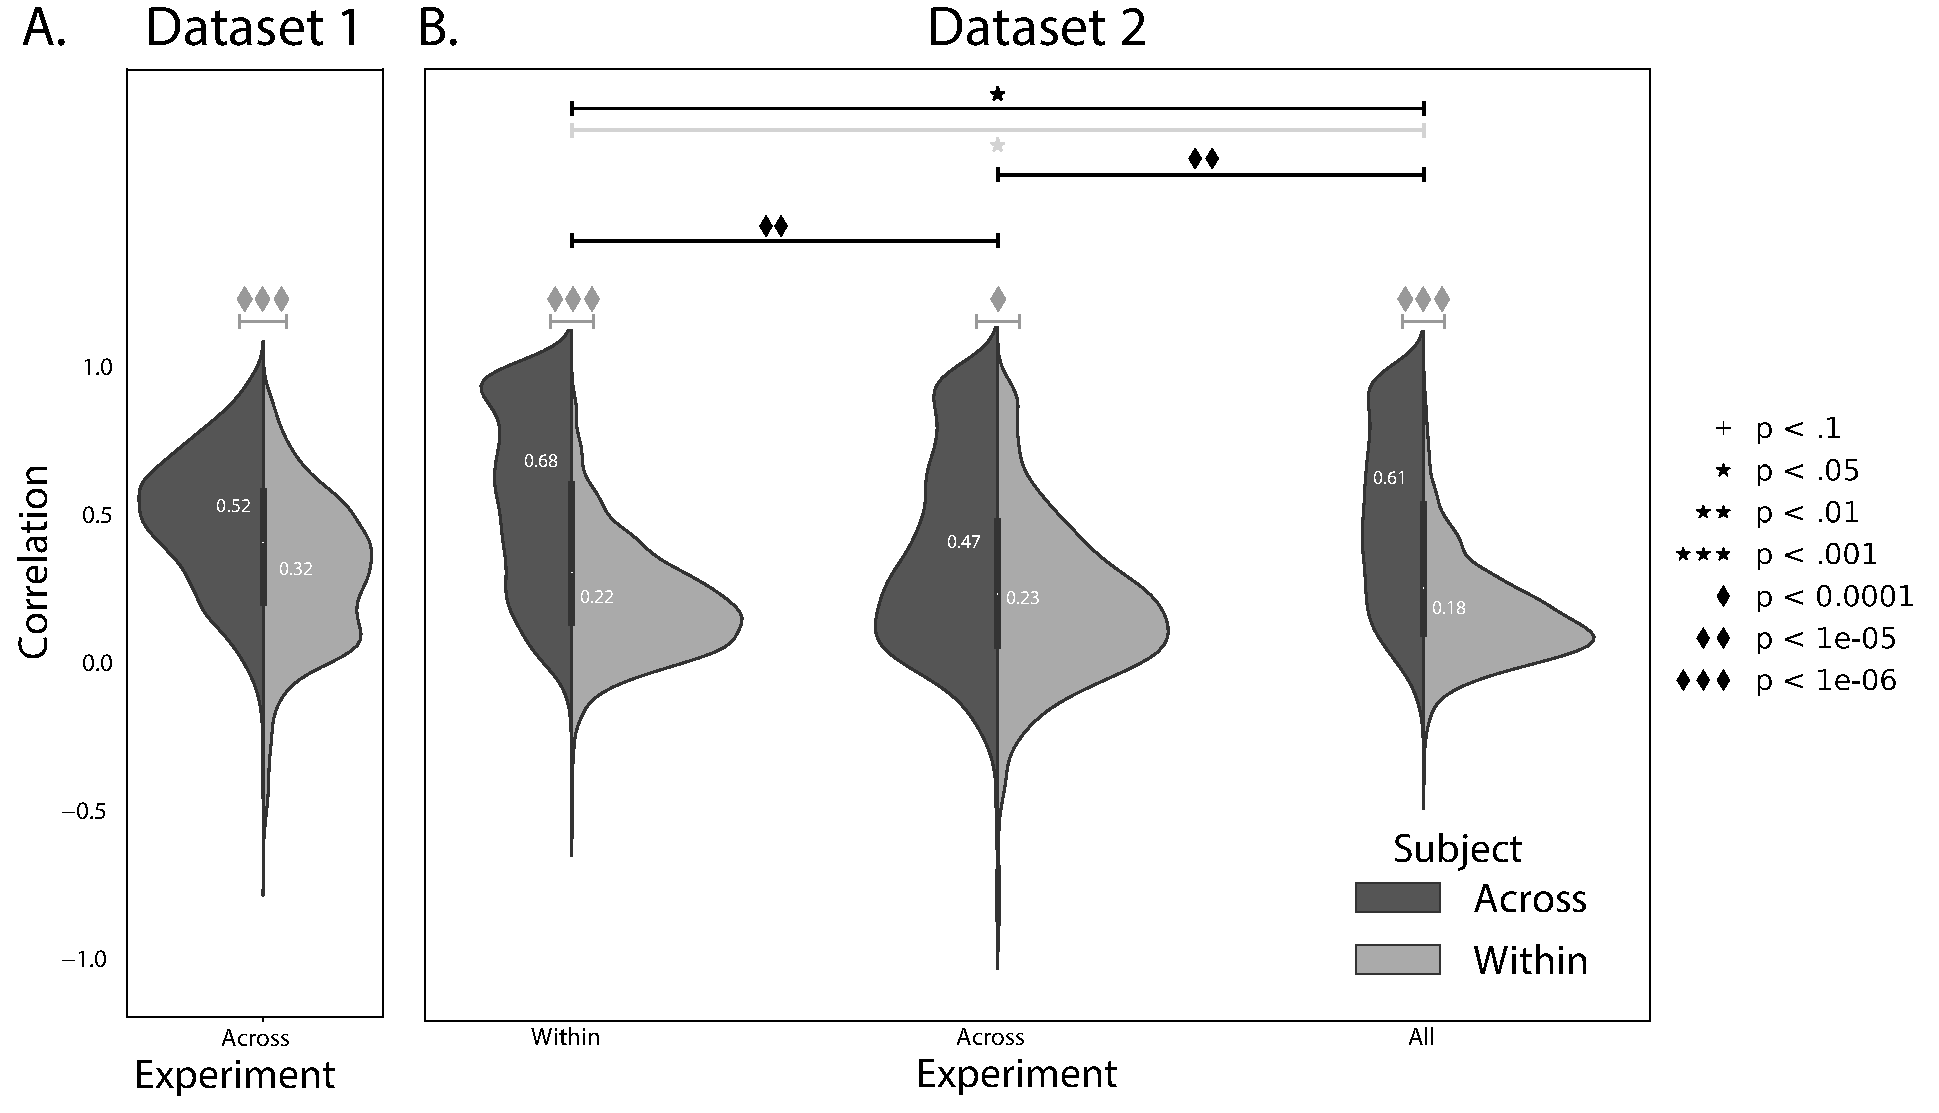
\includegraphics[width=\textwidth]{figs/supplemental_1}
\caption{\textbf{Reconstruction quality across all electrodes in two
    ECoG datasets, broken down by experiment.}
  \textbf{A. Distributions of correlations between observed versus
    reconstructed activity by electrode, for Dataset 1.}  The
  across-patient distribution (black) reflects reconstruction accuracy
  (correlation) using a correlation model learned from all but one
  patient's data, and then applied to that held-out patient's data.
  The within-patient distribution (gray) reflects performance using a
  correlation model learned from the same patient who contributed the
  to-be-reconstructed electrode.  The split violin plot displays the
  same distributions shown in Figure~\corrmaps A.
  \textbf{B. Distributions of correlations for Dataset 2.}  The split
  violin plots are in the same format as those in Panel A.  The
  leftmost plot (``Within'') displays the same distributions shown in
  Figure~\corrmaps B.  All reconstructions reflected in the
  distribution were carried out using a model trained and tested using
  data from the same experiment.  The middle plots (``Across'')
  reflect reconstructions trained and tested using data from different
  experiments.  The rightmost plot (``All'') reflect reconstructions
  obtained using models trained and tested on data from both
  experiments.  The black distributions reflect models trained and
  tested across patients (analogous to the black histograms in
  Figure~\corrmaps) and the gray distributions reflect models trained
  and tested within patient (analogous to the gray histograms in
  Figure~\corrmaps).  The dark gray significance bars reflect
  paired-sample $t$-tests comparing the ($z$-transformed)
  reconstruction accuracy for each electrode obtained within versus
  across patients.  The black significance bars reflect paired-sample
  $t$-tests comparing the across-patient reconstruction accuracies
  across datasets.  The light gray significance bars reflect
  paired-sample $t$-tests comparing the within-patient reconstruction
  accuracies across datasets.  The symbols denote the corresponding
  $p$-values of those statistical tests.}
\label{fig:supplemental_1}
\end{figure}


\begin{figure}[p]
\centering
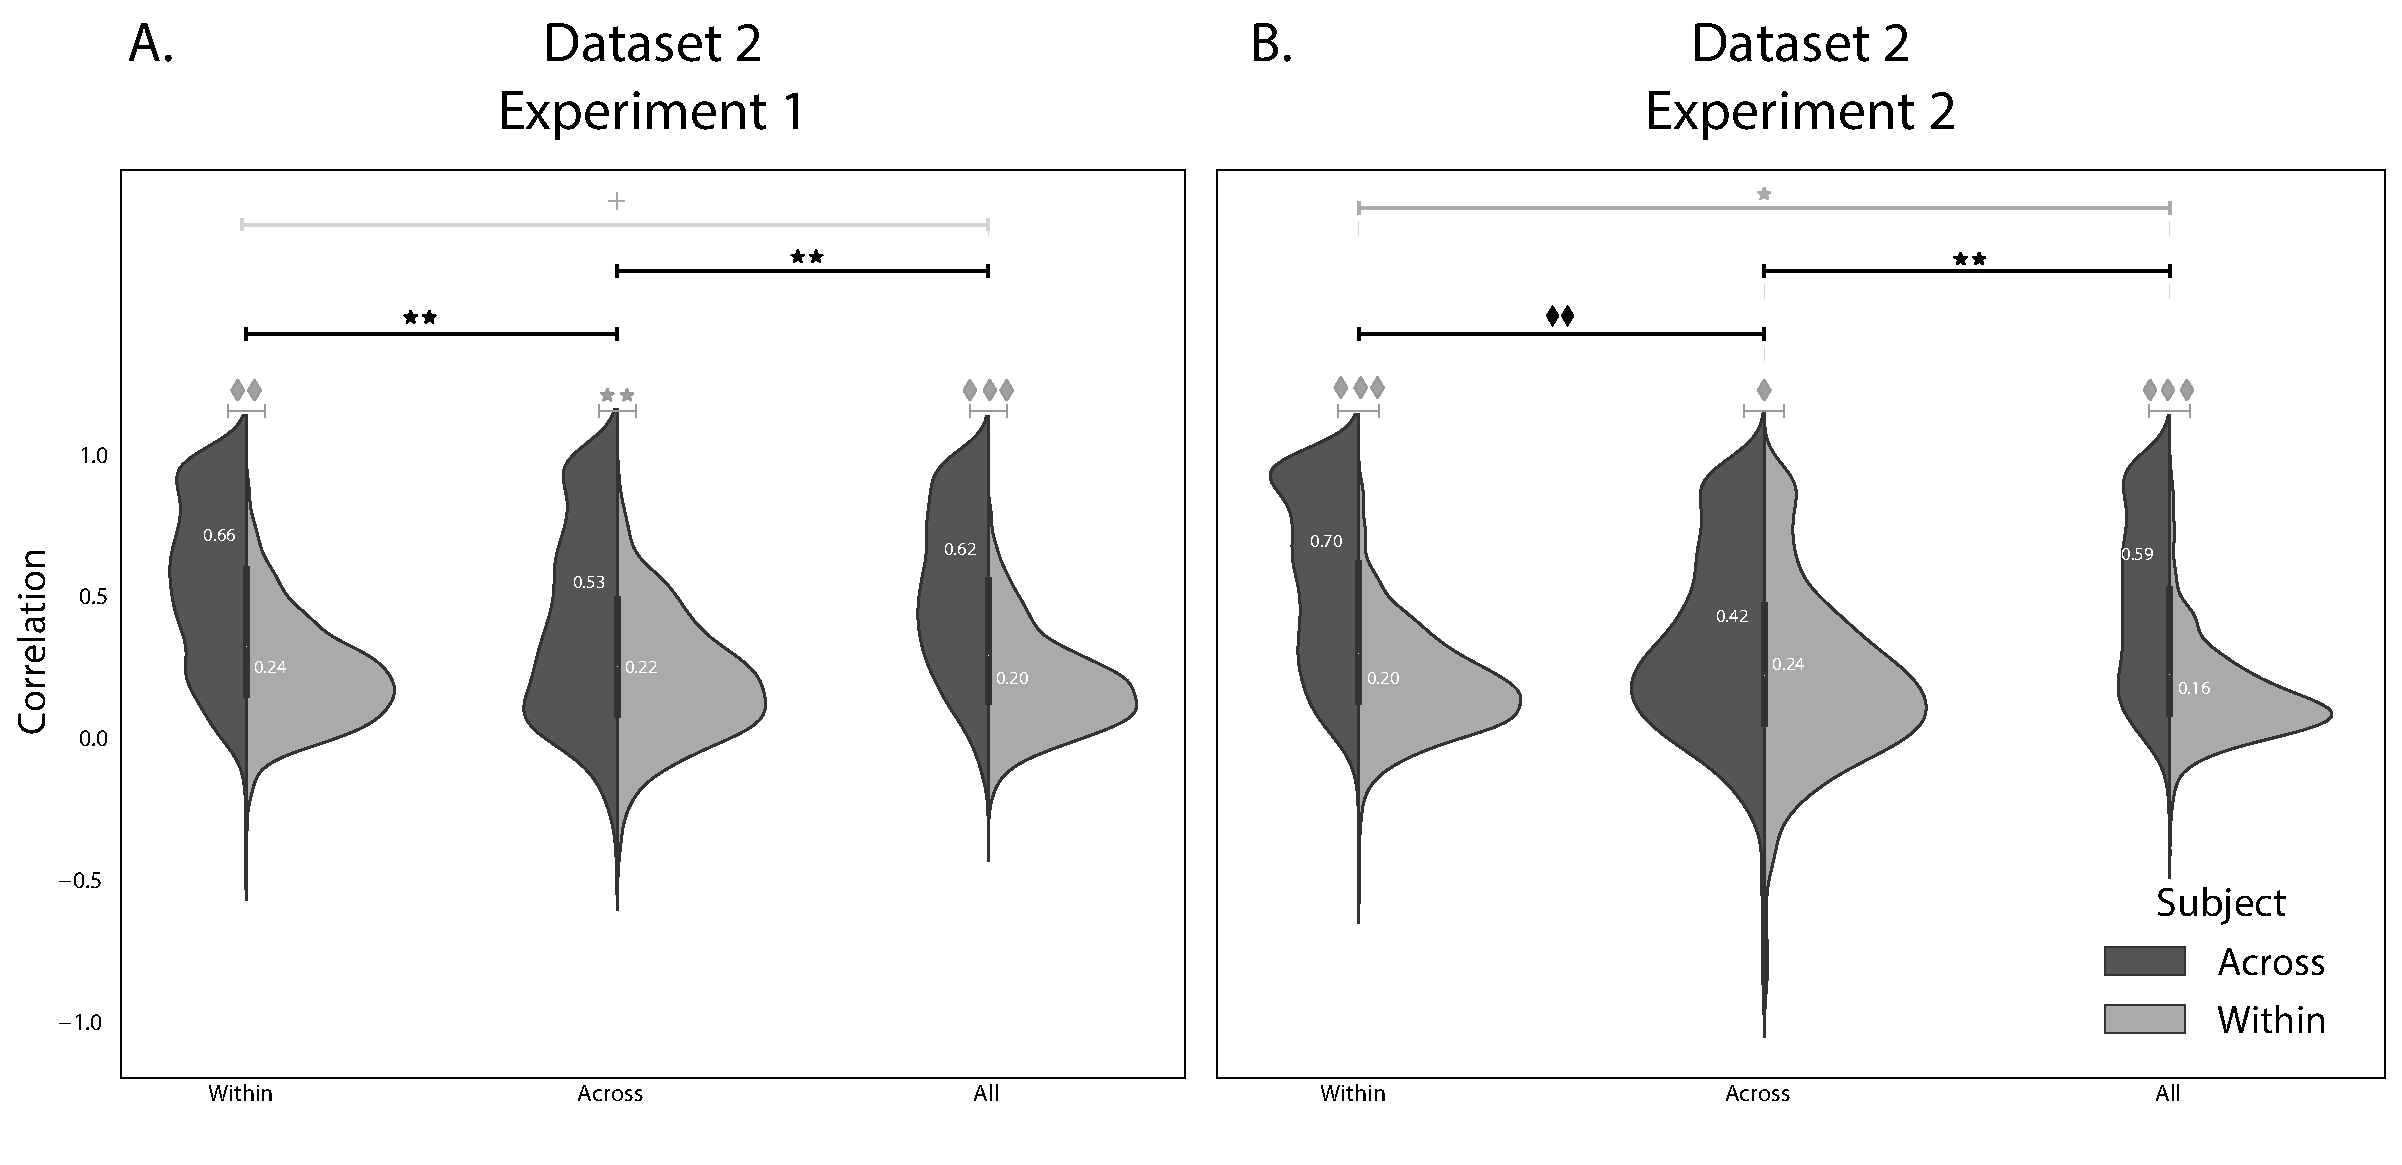
\includegraphics[width=\textwidth]{figs/supplemental_2}
\caption{\textbf{Reconstruction quality for Dataset 2, Experiments 1
    and 2.}  \textbf{A. Distributions of correlations between observed
    versus reconstructed activity by electrode, for Dataset 2
    (Experiment 1).}  The plots are in the same format as
  Figure~\ref{fig:supplemental_1}B, but reflect data only from
  Experiment 1 in Dataset 2.  \textbf{A. Distributions of correlations between observed
    versus reconstructed activity by electrode, for Dataset 2
    (Experiment 2).  The plots are in the same format as Panel A, but
    reflect data only from Experiment 2 in Dataset 2.}}
% \label{fig:supplemental_2}
% \end{figure}
%
% %JRM STOPPED HERE
% \begin{figure}[p]
% \centering
% 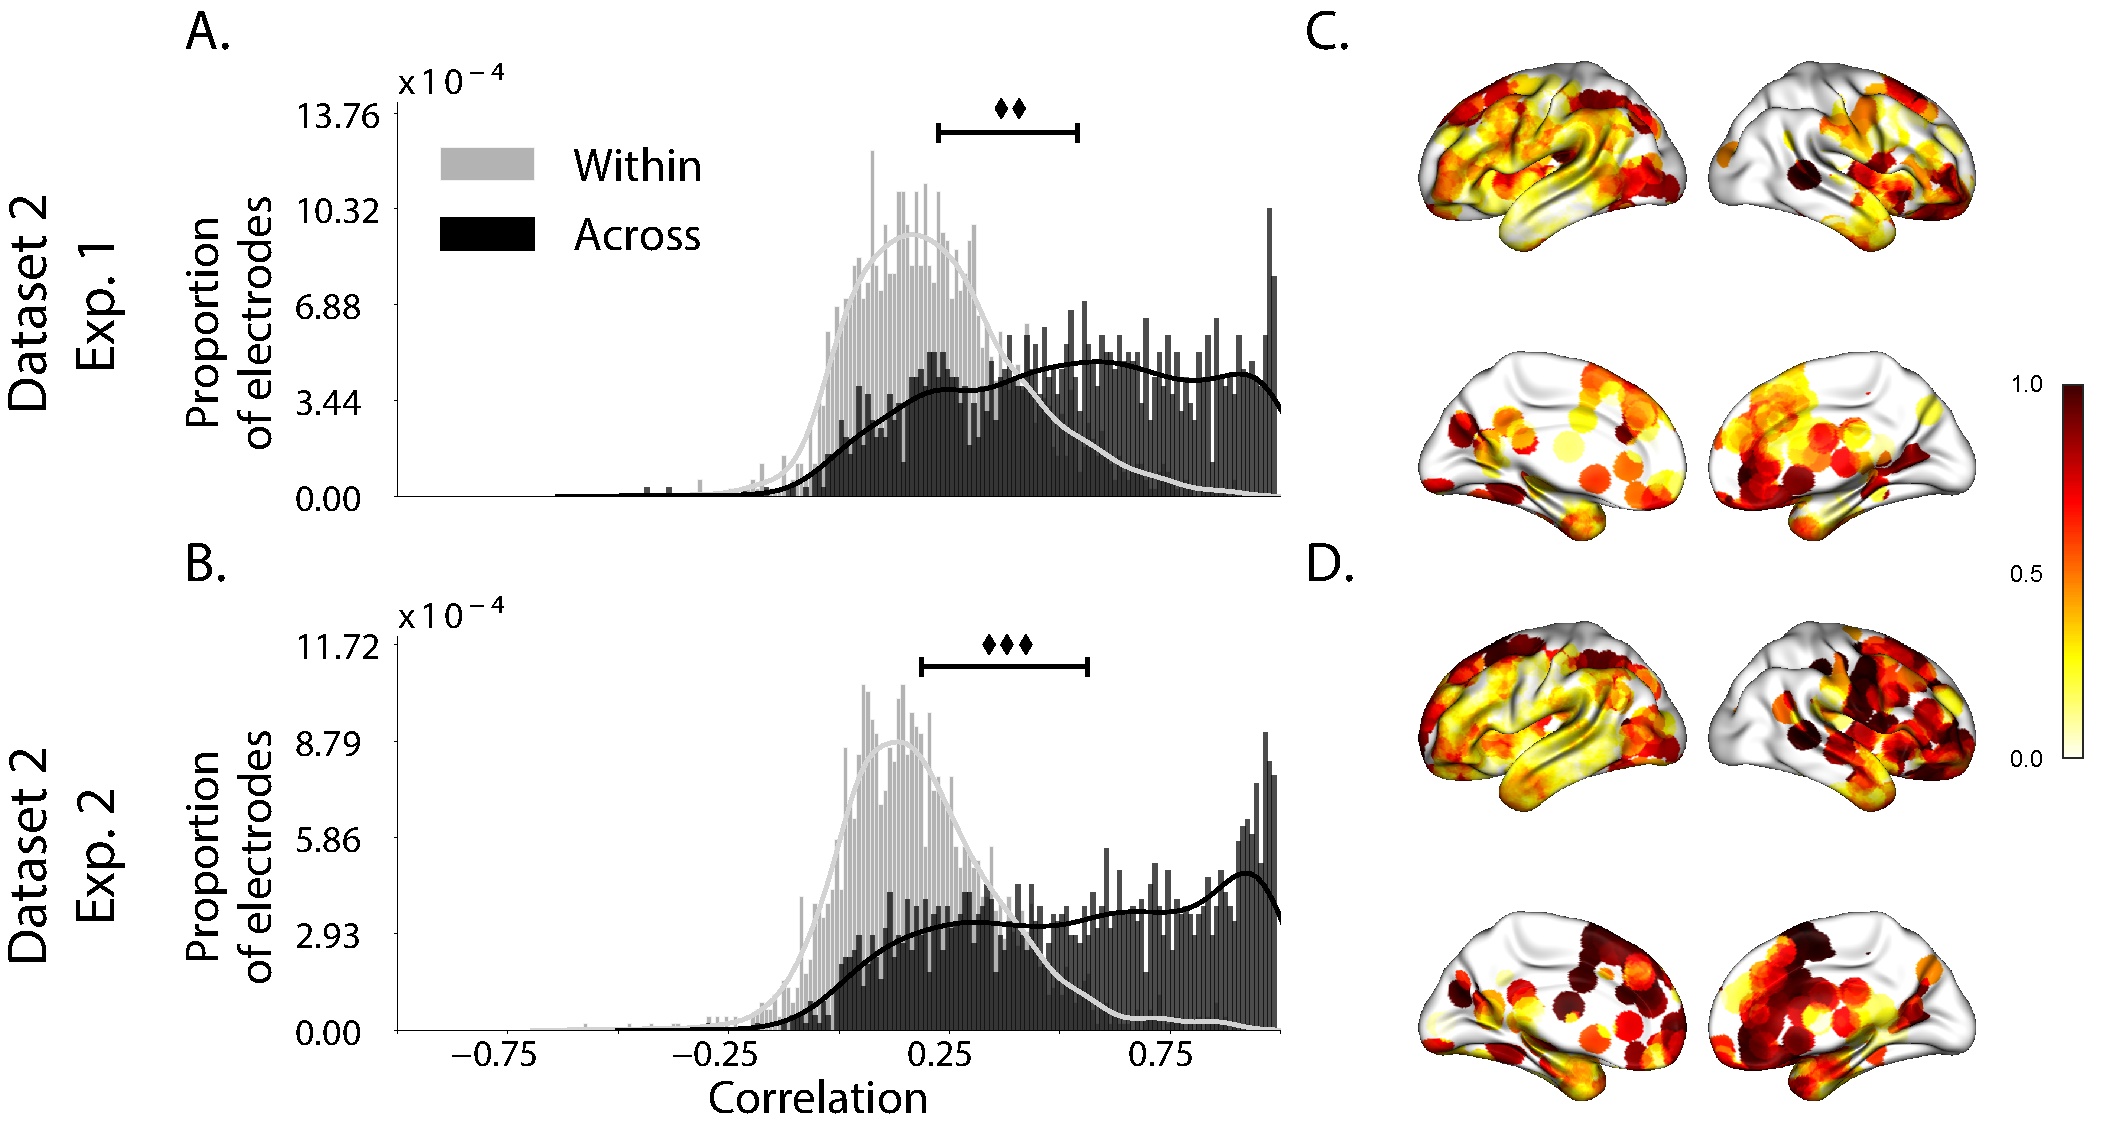
\includegraphics[width=\textwidth]{figs/supplemental_3}
% \caption{\textbf{Reconstruction quality across all electrodes, broken
%     down by Dataset 2 experiment.}  \textbf{A. Distributions of correlations
%       between observed versus reconstructed activity by electrode, for
%       Dataset 1.}  The across-patient distribution (black) reflects
%     reconstruction accuracy (correlation) using a correlation model
%     learned from all but one patient's data, and then applied to that
%     held-out patient's data.  The within-patient distribution (gray)
%     reflects performance using a correlation model learned from the same
%     patient who contributed the to-be-reconstructed electrode.
%     \textbf{B. Distributions of correlations for Dataset 2.}  This
%     panel is in the same format as Panel A, but reflects results
%     obtained from Dataset 2.  The histograms aggregate data across
%     both Dataset 2 experiments; for results broken down by experiment
%     see Figure~\perexptaskreconseparated. \textbf{C.--D.  Reconstruction
%       performance by location.} The colors denote the average across-session
%     correlation, using the across-patient correlation model, between
%     the observed and reconstructed activity at the given electrode
%     location projected to the cortical surface~\citep{CombEtal19}.}
%
%
% \caption{\textbf{Reconstruction quality across all electrodes in two
%       Dataset 2 experiments.}  \textbf{A. Distributions of correlations
%       between observed versus reconstructed activity by electrode, for
%       Experiment 1.}  Same format as Figure~3A and B, but reflects data shown
%     in Figure~\ref{fig:supplemental_2}A (leftmost violin plot).
%  \textbf{B. Distributions of correlations
%       between observed versus reconstructed activity by electrode, for
%       Experiment 2.}  Same format as Figure~3A and B, but reflects
%     data shown in Figure~\ref{fig:supplemental_2}B (leftmost violin
%     plot).  \textbf{C.--D.  Reconstruction
%       performance by location.} Each dot reflects the location of a
%     single implanted electrode from Dataset 2, Experiment 1 (Panel C)
%     or Dataset 2, Experiment 2 (Panel D).  The dot colors denote the
%     average within-experiment (across-session)
%     correlation, using the across-patient correlation model, between
%     the observed and reconstructed activity at the given electrode
%     location projected to the cortical surface~\citep{CombEtal19}.}
\label{fig:supplemental_3}
\end{figure}



\begin{figure}[p]
\centering
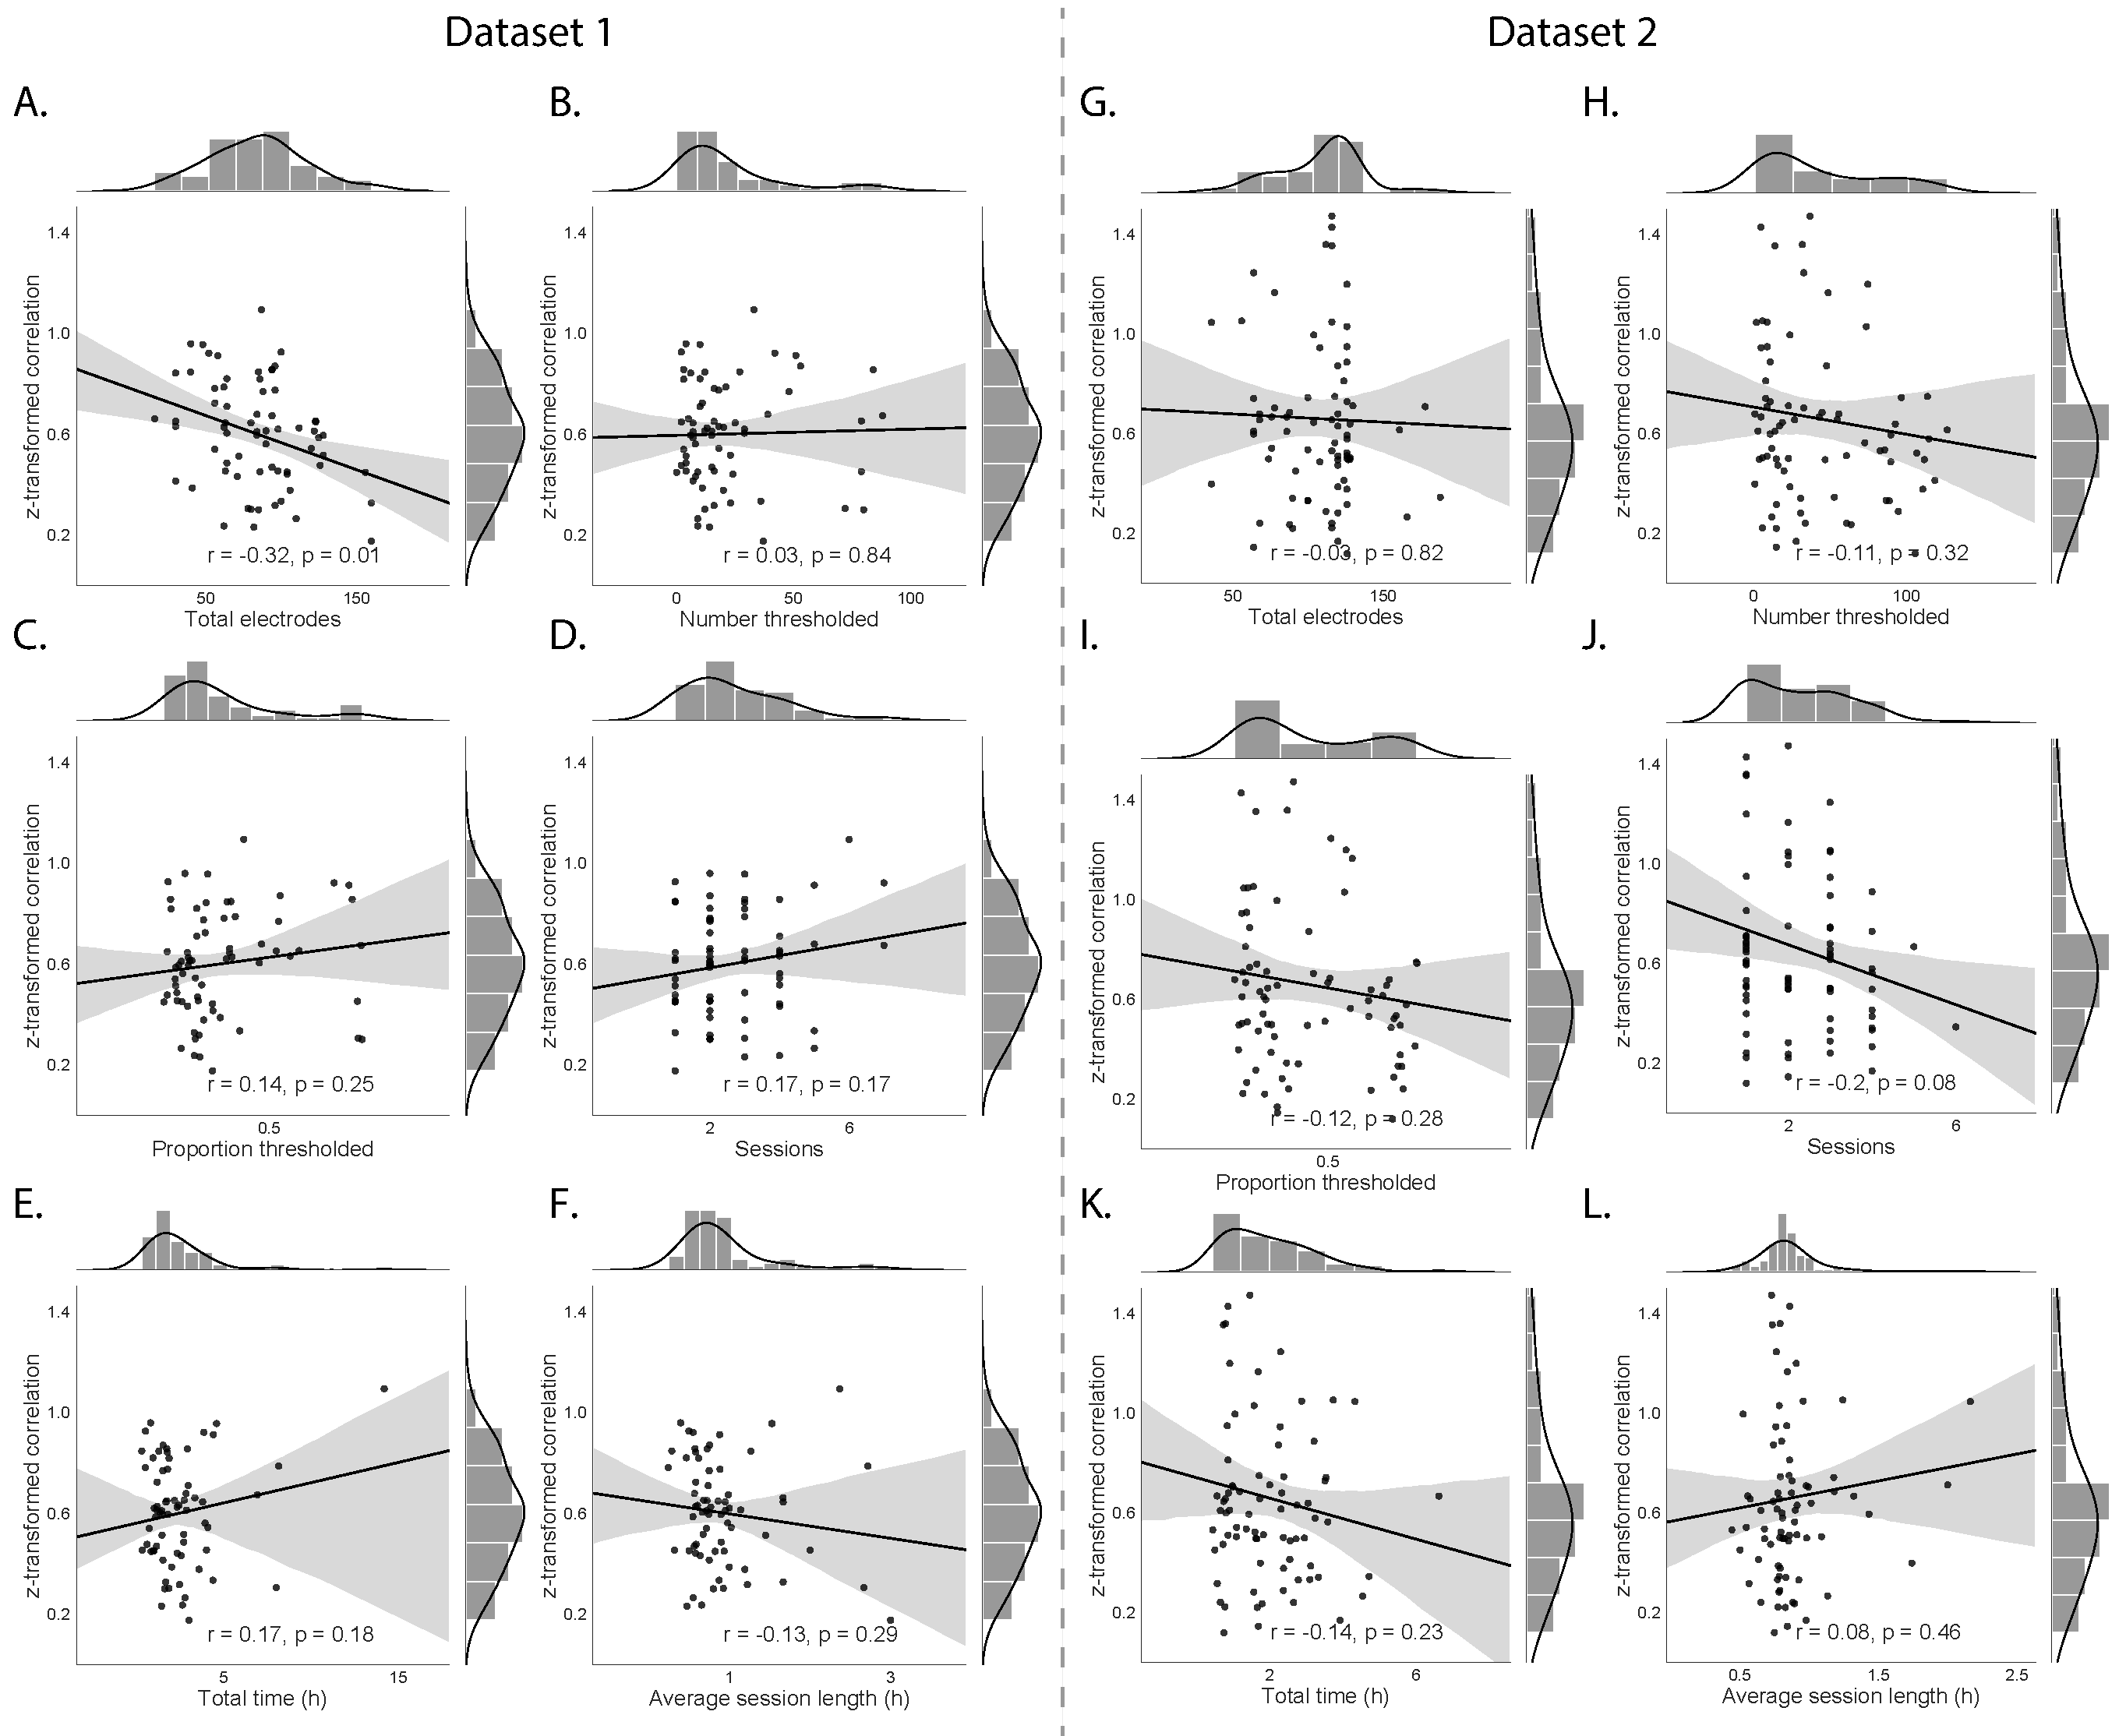
\includegraphics[width=\textwidth]{figs/supplemental_4}
\caption{\textbf{Reconstruction quality across all electrodes in two
      ECoG datasets for each frequency band.} \textbf{A. Distributions of correlations
      between observed versus reconstructed activity by electrode, for
      each frequency band in Dataset 1.} Same format as Figure~5A, but
    using power at each frequency.
    \textbf{B.~Statistical summary of across-patient reconstruction
      quality by electrode for each frequency band in Dataset 1.} Same format as Figure~5B, but
    using power at each frequency.\textbf{C.~Statistical summary of within-patient reconstruction
      quality by electrode for each frequency band in Dataset 1.}
    This panel displays the within-patient statistical summary,
    in the same format as Panel B.  \textbf{D.~Distributions of correlations
      between observed versus reconstructed activity by electrode, for
      each frequency band in Dataset 2.}  This panel displays
    reconstruction accuracy distributions for each frequency band for
    Dataset 2. \textbf{E.~Statistical summary of
      across-patient reconstruction quality by electrode for each
      frequency band in Dataset 2.} This is the same format as Panel
    B for Dataset 2. \textbf{F.~Statistical summary of
      within-patient reconstruction quality by electrode for each
      frequency band in Dataset 2.}This is the same format as Panel
    C for Dataset 2.}
\label{fig:supplemental_4}
\end{figure}

\begin{figure}[p]
\centering
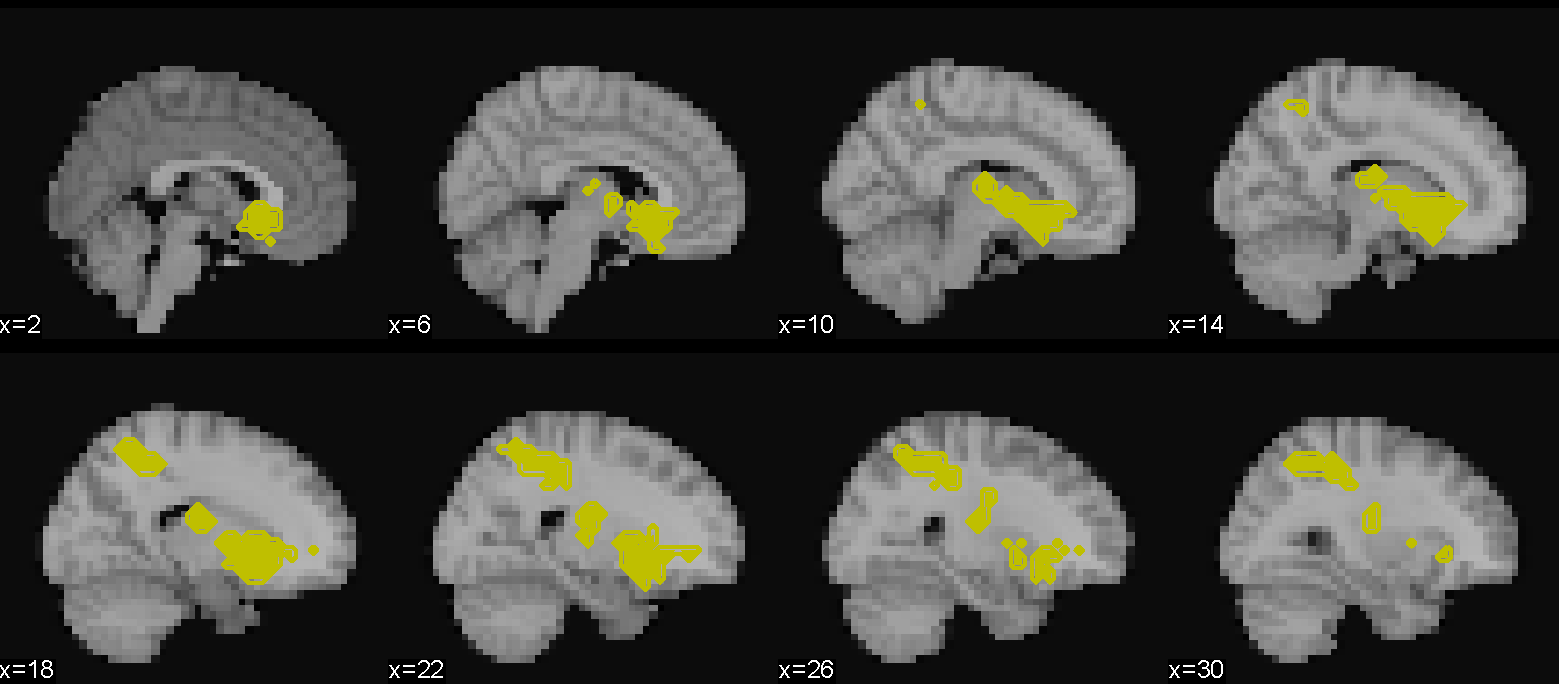
\includegraphics[width=\textwidth]{figs/supplemental_5}
\caption{\textbf{Most informative electrode locations by frequency
      and the networks involved.}
    \textbf{A.~Intersections across datasets for each frequency.}  Same format as Figure~6A, but
    using power at each frequency.
    \textbf{B.~Proportion of networks in most informative electrode locations by
    frequency.}  Pie graphs display the proportion of the 7 networks
  ~\citep{YeoEtal11} in the most informative locations by
  frequency, and are sized relative to the average reconstruction
  accuracy for each frequency. \textbf{C.~Terms associated with most informative
    electrode locations.}  The
    lists of terms display the top five Neurosynth
    terms~\citep{RubiEtal17} decoded from the corresponding brain
    maps, and colored according the frequency (see Panel
    E legend). \textbf{D.~Network parcellation from~\citep{YeoEtal11}.}
    Seven network parcellation as described
    in~\citep{YeoEtal11}. \textbf{E.~Most informative locations by
      frequency.} The inflated brain plot displays the locations of
    the most informative locations (Panel A), colored by frequency,
    and projected onto the cortical surface~\citep{CombEtal19}.}
\label{fig:supplemental_5}
\end{figure}

\begin{figure}[p]
\centering
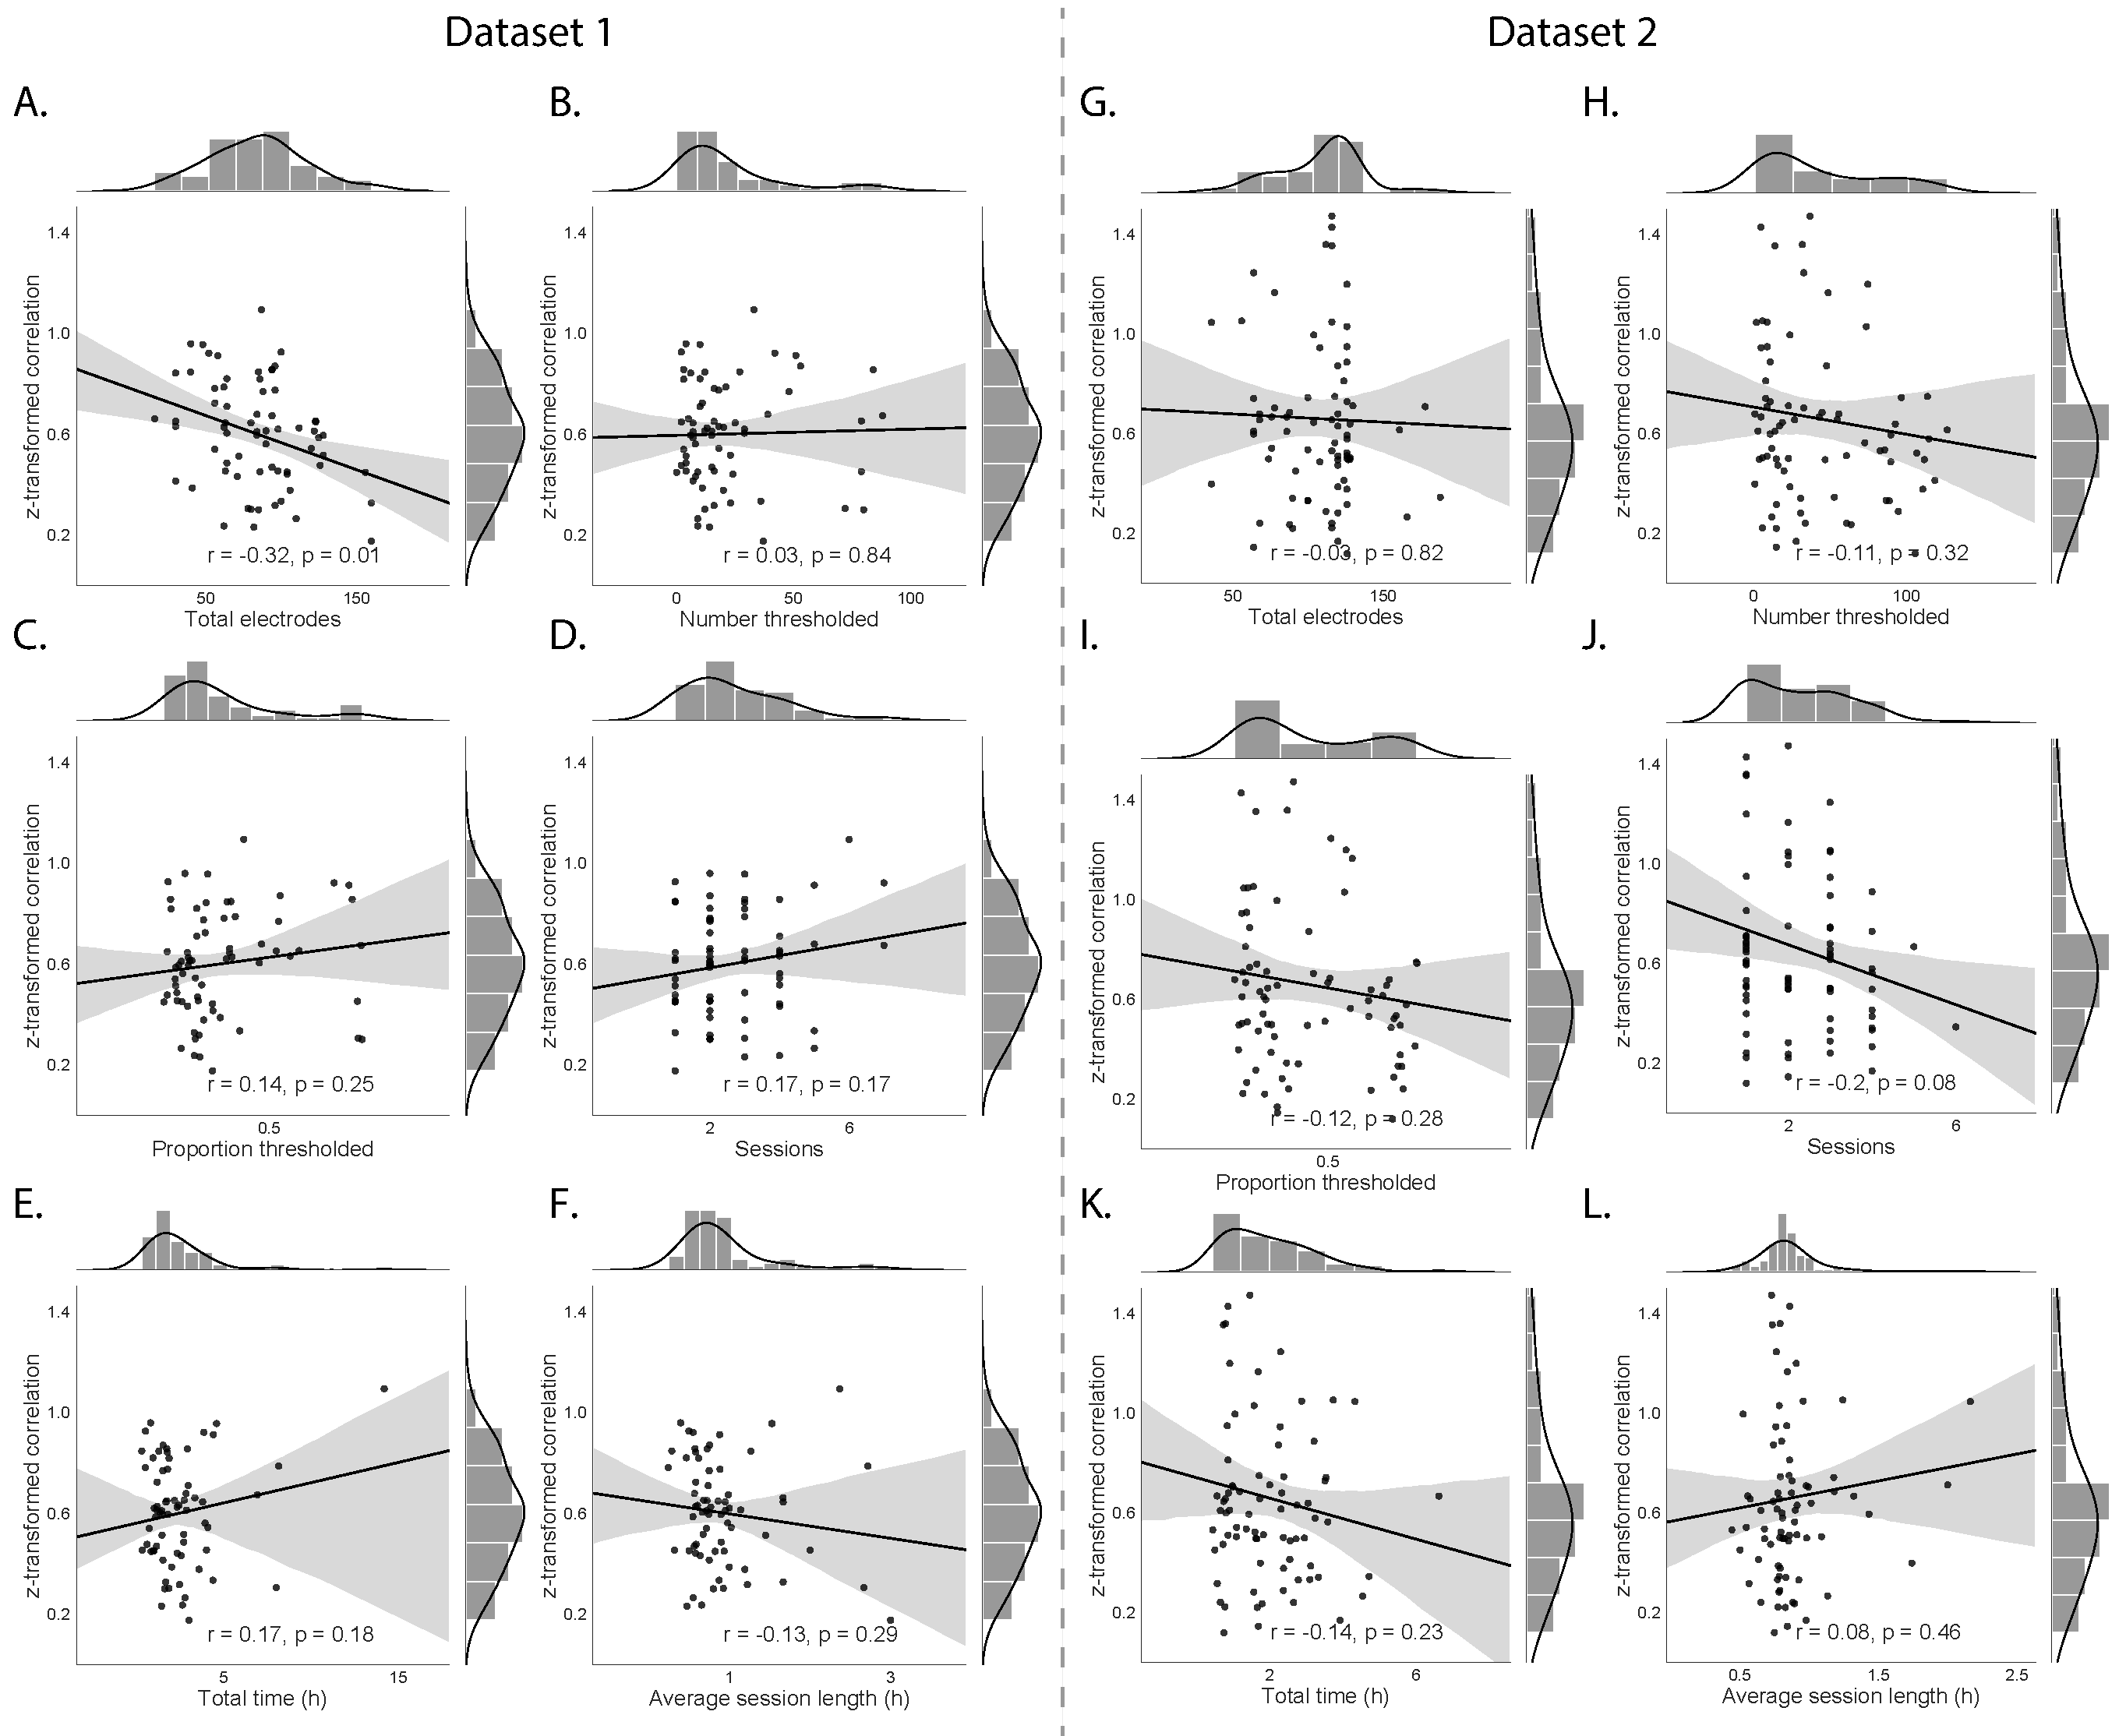
\includegraphics[width=\textwidth]{figs/supplemental_6}
\caption{\textbf{Reconstruction accuracy versus within-subject data
    features for two ECoG datasets.} \textbf{A.--F.  Features from
    Dataset 1.}  Features include: (\textbf{A.}) total number of
  electrodes implanted in each patient's brain, (\textbf{B.})
  per-patient number of electrodes that were filtered out due to
  having an maximum kurtosis greater than 10 across all recording
  sessions, (\textbf{C.})  per-patient proportion of electrodes that
  were filtered out due to having an average kurtosis greater than 10,
  (\textbf{D.})  per-patient number of recording sessions,
  (\textbf{E.}) per-patient total recording time (h), and
  (\textbf{F.}) per-patient average session length (h).
  \textbf{G.--L. Features from Dataset 2.}  Analogous format to Panels
  A--F.}
\label{fig:supplemental_6}
\end{figure}

\begin{figure}[p]
\centering
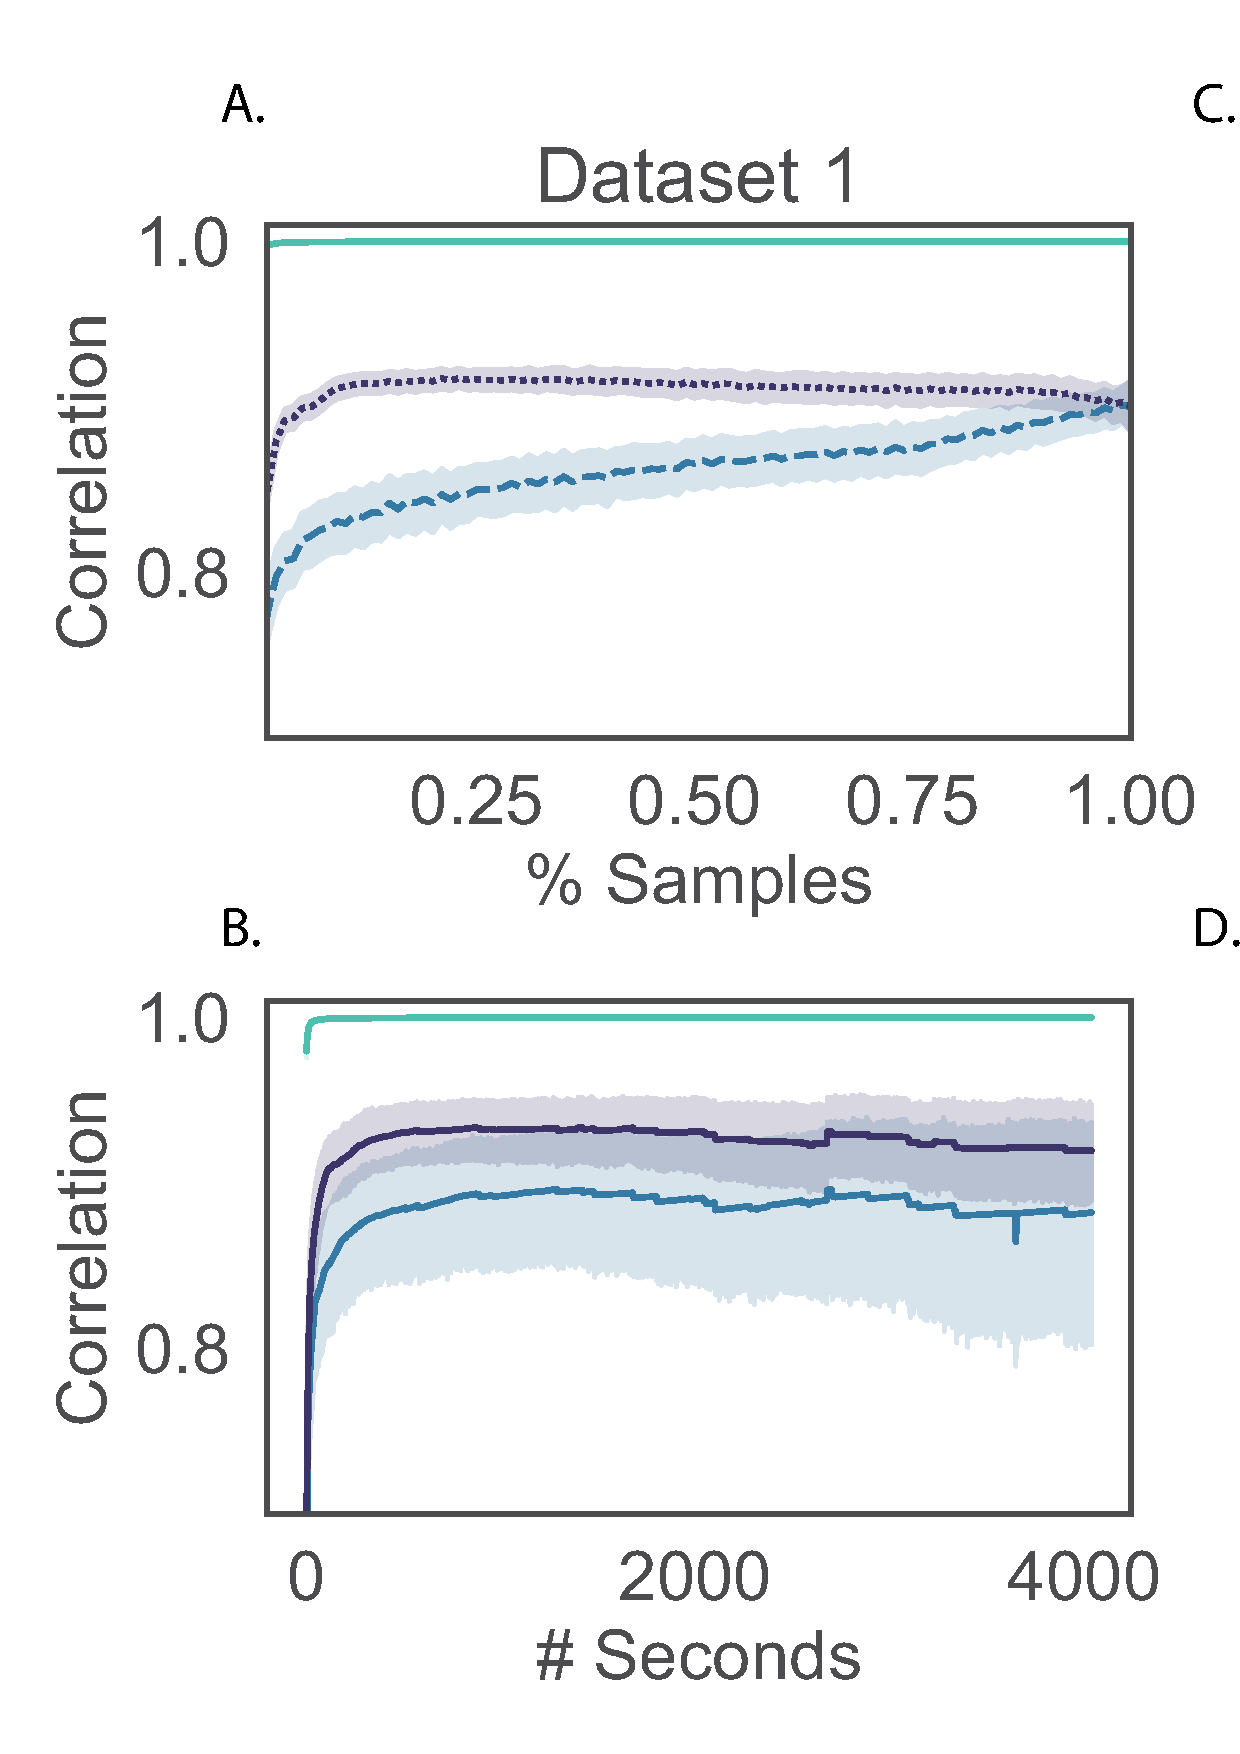
\includegraphics[width=\textwidth]{figs/supplemental_7}
\caption{\textbf{Stability of correlation matrix across time.} \textbf{A.--B.  Features from
    Dataset 1.}  Features include: (\textbf{A. Correlation of split
  halves by the percent samples included.})  For each patient, we
  split the timeseries data in
  half and created a correlation matrix with one half.  With the
  remaining data, we created the second correlation matrix with more
  and more time samples (in 1000 sample increments).  These time
  samples were either drawn randomly (``Random'') , or were drawn sequentially from
  either the closest timepoint (``Close'' ) or the furthest timepoint
  (``Apart'' ). The two correlation matrices were then correlated, and the
  coefficient plotted relative to the percentage of data included.  (\textbf{B. Correlation of split
  halves by the number of time samples included.})
Same analysis as Panel A, but the
  coefficient plotted relative to the total number of samples included.
  \textbf{C.--D. Features from Dataset 2.}  Analogous format to Panels
  A--B.}
\label{fig:supplemental_7}
\end{figure}

\begin{figure}[p]
\centering
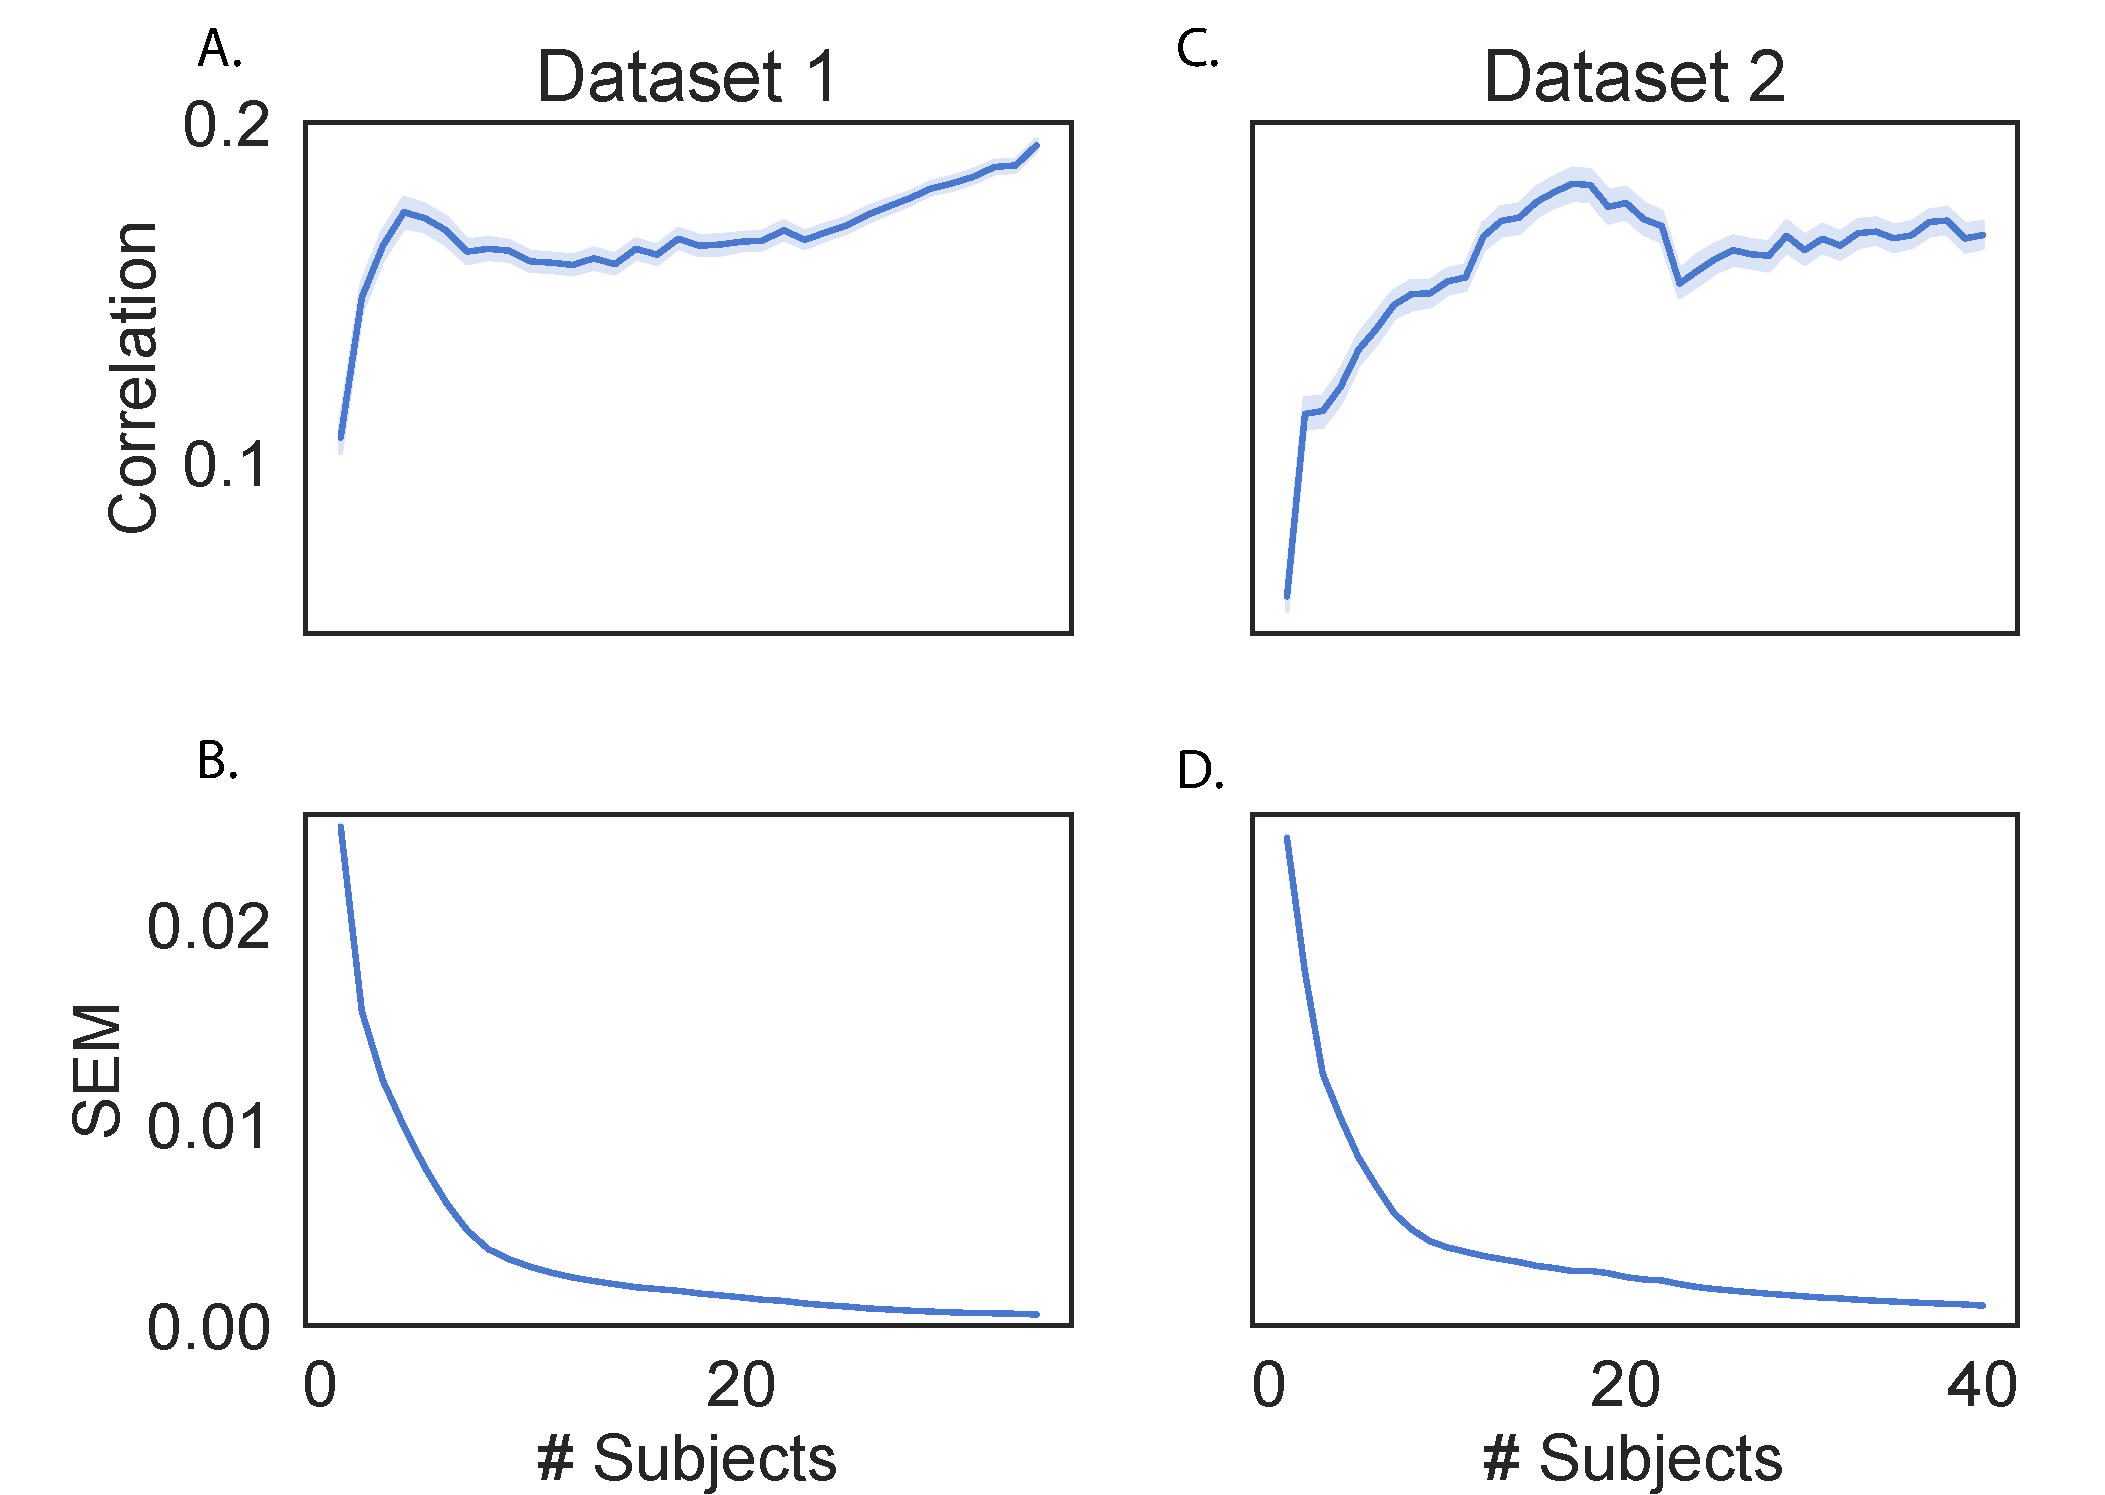
\includegraphics[width=\textwidth]{figs/supplemental_8}
\caption{\textbf{Stability of correlation matrix across patients.} \textbf{A.--B.  Features from
    Dataset 1.}  Features include: (\textbf{A. Correlation of split
  halves by number of patients included.})  For 500 iterations, we randomly split the
patient-specific correlations in half, then created one correlation
matrix with the first half and created the second correlation matrix
using more and more patients. The two correlation matrices were then correlated, and the
  coefficient plotted relative to the number of patients included.
  (\textbf{B. Standard error of the mean across iterations by the
    number of patients included.})
To measure the variability across the iterations, we plot the standard
error of the mean as a function of the number of patients included in
the second correlation matix.
  \textbf{C.--D. Features from Dataset 2.}  Analogous format to Panels
  A--B.}
\label{fig:supplemental_8}
\end{figure}

\clearpage
\newpage
\renewcommand{\bibnumfmt}[1]{[S#1]}
\renewcommand{\citenumfont}[1]{S#1}
\bibliography{CDL-bibliography/memlab}
\bibliographystyle{CSE}
% \newpage
% \renewcommand{\refname}{Supplemental references}
% \bibliography{memlab}


\end{document}
